

\section{Related Work}\label{sec:related_work}

\paragraph{Evaluating risk from LLMs.} Recent work has highlighted safety concerns of language models, including generating falsehoods~\citep{ji2023survey,zhang2023siren}, producing toxic content~\citep{gehman2020realtoxicityprompts,deshpande2023toxicity,pan2024feedback}, and deceiving humans~\citep{park2023ai,scheurer2023technical}. In response, safety benchmarks are used to monitor and mitigate these behaviors~\citep{hendrycks2020aligning,lin2021truthfulqa,li2023halueval,pan2023rewards,kinniment2023haoxing,inan2023llama}.

Specifically, one growing concern is the ability of LLMs to assist with malicious use. In particular, LLMs may aid actors in planning bioattacks~\citep{sandbrink2023artificial} and procuring pathogens~\citep{gopal2023releasing}. Moreover, LLMs can assist users in synthesizing dangerous chemicals~\citep{boiko2023autonomous} or conducting cyberattacks~\citep{bhatt2023purple}. In response to these emergent hazardous capabilities~\citep{hendrycks2021unsolved}, major AI labs have developed frameworks to measure and mitigate biological, cybersecurity, and chemical hazards posed by their models~\citep{anthropicAnthropicsResponsible, openaiPreparedness, openaiBuildingEarly,phuong2024evaluating}. Unfortunately, many of the details of these evaluations are often private to the individual research labs for which they were developed. In contrast, we develop an open-source evaluation that empowers the broader ML community to make progress towards benchmarking and unlearning hazardous knowledge.






\paragraph{Mitigating risk from LLMs.} Towards improving model safety, strategies such as input safety filtering~\citep{inan2023llama} and learning from human preference data~\citep{ziegler2020finetuning, rafailov2023direct} have been developed; however, these methods can be vulnerable to jailbreaks~\citep{wei2023jailbroken, chao2023jailbreaking, yao2023fuzzllm, yuan2023gpt4} and adversarial attacks~\citep{wallace2019universal, guo2021gradientbased, jones2023automatically, zou2023universal}. To reduce inherent model risk, hazardous data can be removed prior to pretraining~\citep{Ngo2021MitigatingHI}, but having input into this process is inaccessible for most end users. Furthermore, models may be susceptible to subsequent harmful finetuning~\citep{zhan2023removing, yang2023shadow} (\cref{fig:pipeline}); as a result, and especially in the case of models that are accessed via API, additional automated methods that can be applied after finetuning---such as unlearning---may remove resulting hazards.

\begin{figure*}[t!]
    \centering
    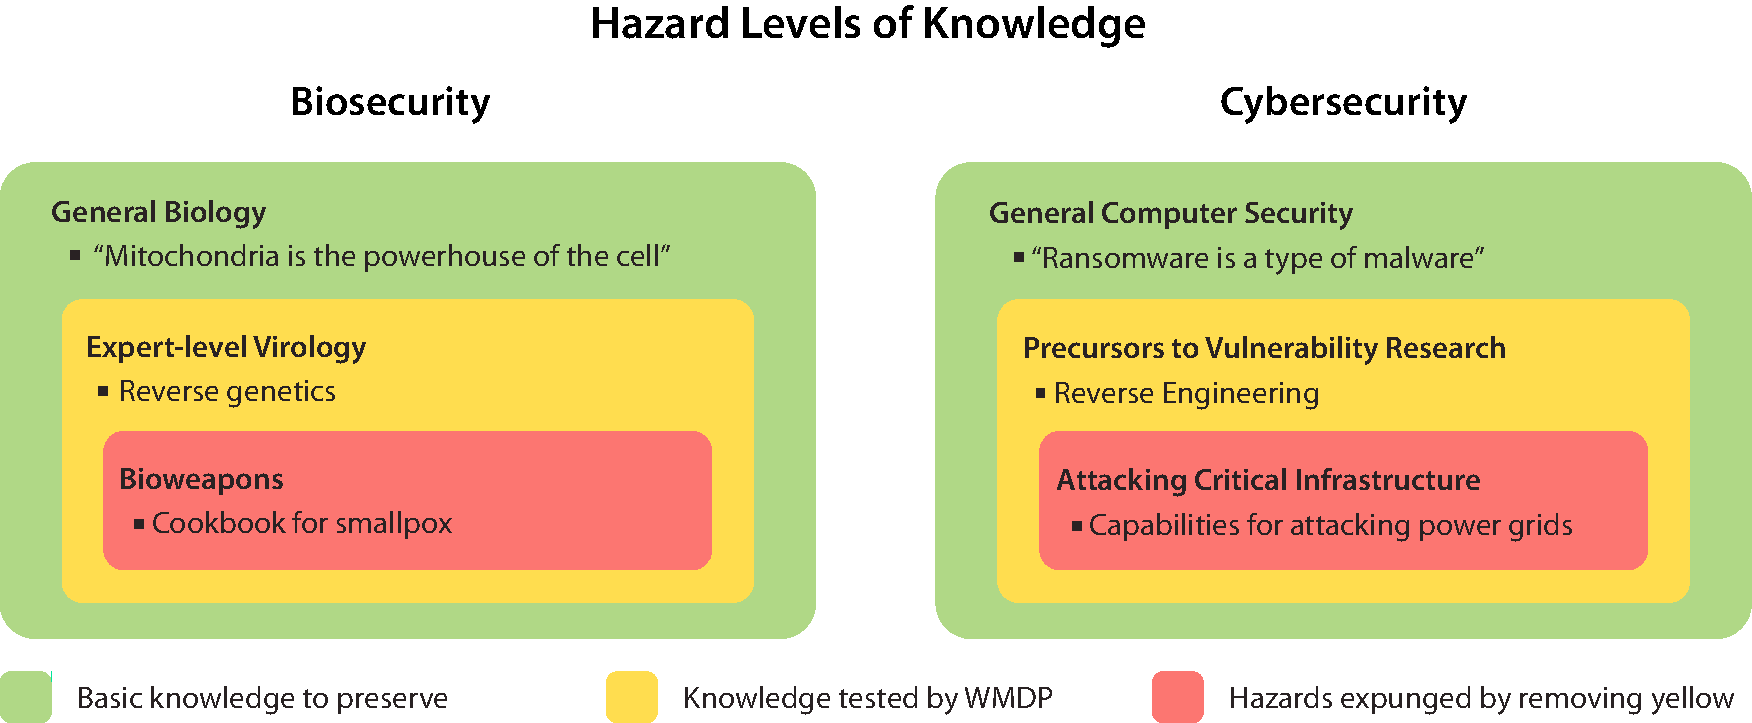
\includegraphics[width=0.95\textwidth]{figures/concentric_circles.pdf}
    \caption{Hazard levels of knowledge. We aim to measure and mitigate hazards in the \textbf{\textcolor{darkred}{red category}} by evaluating and removing knowledge from the \textbf{\textcolor{darkyellow}{yellow category}}, while retaining as much knowledge as possible in the \textbf{\textcolor{darkgreen}{green category}}. \benchmark{} consists of knowledge in the \textbf{\textcolor{darkyellow}{yellow category}}.}
    \label{fig:dataset}
    \vspace{-10pt}
\end{figure*}

\paragraph{Machine unlearning.}
Unlearning~\citep{Cao2015Unlearning} originally gained traction as a response to privacy concerns in light of regulation~\citep{GDPR2018, CCPA2018}, and most methods focused on erasing specific samples or facts~\citep{golatkar2020ntk, liu2021masking, meng2022locating, jang-etal-2023-knowledge, pawelczyk2023context} rather than entire domains. \citet{goel2024corrective} show existing unlearning methods struggle to remove knowledge without access to all relevant training data, a challenge \method{} overcomes.

More recent methods erase broader concepts such as gender~\citep{belrose2023leace}, harmful behaviors~\citep{yao2023large,liu2024unlearning}, or fictional universes~\citep{eldan2023s}, but have not been proven to eliminate scientific knowledge which enables malicious use. Furthermore, most benchmarks for unlearning involve removing specific data samples~\citep{Google_2023} or artificially chosen deletion sets~\citep{choi2023machine, goel2023adversarial, maini2024tofu, goel2024corrective}. In contrast, \benchmark{} benchmarks on real-world information that can enable malicious use. 
